% Standard model of physics
% Author: Carsten Burgard
\documentclass[border=10pt]{standalone}
\usepackage{tikz}
\usetikzlibrary{calc,positioning,shadows.blur,decorations.pathreplacing}
\usepackage{etoolbox}

\tikzset{%
        brace/.style = { decorate, decoration={brace, amplitude=5pt} },
       mbrace/.style = { decorate, decoration={brace, amplitude=5pt, mirror} },
        label/.style = { black, midway, scale=0.5, align=center },
     toplabel/.style = { label, above=.5em, anchor=south },
    leftlabel/.style = { label,rotate=-90,left=.5em,anchor=north },   
  bottomlabel/.style = { label, below=.5em, anchor=north },
        force/.style = { rotate=-90,scale=0.5 },
        round/.style = { rounded corners=2mm },
       legend/.style = { right,scale=0.4 },
        nosep/.style = { inner sep=0pt },
   generation/.style = { anchor=base }
}

%\definecolor{green}{HTML}{B5D99C}
\definecolor{green}{HTML}{c3e0af}
\definecolor{red}{HTML}{EB7876}
\definecolor{lightred}{HTML}{EEA3A1}
\definecolor{yellow}{HTML}{FFFF82}
\definecolor{purple}{HTML}{b4a5d2}
\definecolor{beige}{HTML}{A7C7A8}
\definecolor{grey}{HTML}{808080}
\definecolor{white}{HTML}{FFFFFF}


\newcommand\particle[8][white]{%
  \begin{tikzpicture}[x=1cm, y=1cm]
    \path[fill=#1,blur shadow={shadow blur steps=5}] (0.1,0) -- (0.9,0)
        arc (90:0:1mm) -- (1.0,-0.9) arc (0:-90:1mm) -- (0.1,-1.0)
        arc (-90:-180:1mm) -- (0,-0.1) arc(180:90:1mm) -- cycle;
    \ifstrempty{#7}{}{\path[fill=red]
        (0.5,0) --(0.7,0) -- (1.0,-0.3) -- (1.0,-0.5);}
      \ifstrempty{#8}{}{\path[fill=red]
        (0.5,0) --(0.7,0) -- (1.0,-0.3) -- (1.0,-0.5);}
    \ifstrempty{#6}{}{\path[fill=green] (0.7,0) -- (0.9,0)
        arc (90:0:1mm) -- (1.0,-0.3);}
    \ifstrempty{#5}{}{\path[fill=orange!50!white] (1.0,-0.68) -- (1.0,-0.9)
        arc (0:-90:1mm) -- (0.68,-1.0);}
    \draw[\ifstrempty{#2}{dashed}{black}] (0.1,0) -- (0.9,0)
        arc (90:0:1mm) -- (1.0,-0.9) arc (0:-90:1mm) -- (0.1,-1.0)
        arc (-90:-180:1mm) -- (0,-0.1) arc(180:90:1mm) -- cycle;

    \ifstrempty{#7}{}{\node at(0.8,-0.2) [rotate=-45,scale=0.23,color=white] {\textbf{#7}};}
    \ifstrempty{#8}{}{\node at(0.8,-0.2) [rotate=-45,scale=0.18,color=white] {\textbf{#8}};}
    \ifstrempty{#6}{}{\node at(0.9,-0.1)  [nosep,scale=0.23] {#6};}
    \ifstrempty{#5}{}{\node at(0.9,-0.9)  [nosep,scale=0.23] {#5};}
    \ifstrempty{#4}{}{\node at(0.07,-0.1)  [nosep,anchor=west,scale=0.3]{#4};}
    \ifstrempty{#3}{}{\node at(0.07,-0.85) [nosep,anchor=west,scale=0.35] {#3};}
    \ifstrempty{#2}{}{\node at(0.07,-0.5)  [nosep,anchor=west,scale=1.5] {#2};}
  \end{tikzpicture}
}

\begin{document}
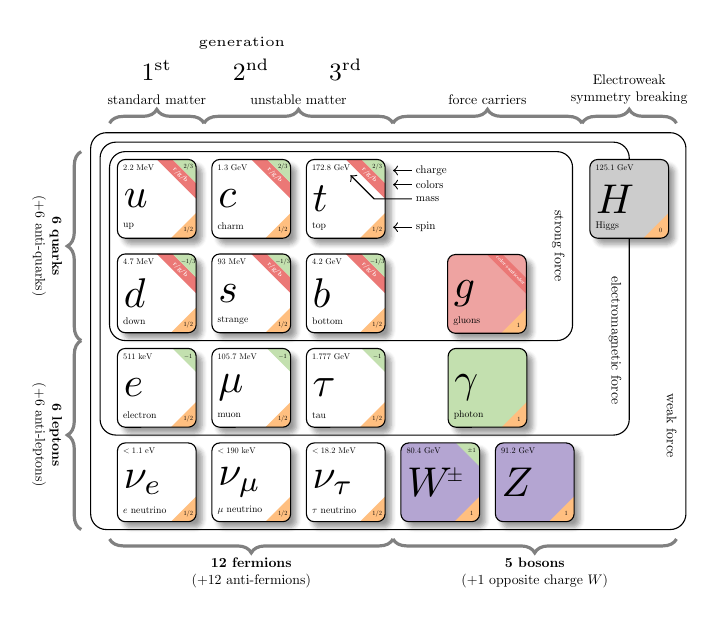
\begin{tikzpicture}[x=1.2cm, y=1.2cm]
  \draw[round] (-0.5,0.5) rectangle (4.4,-1.5);
  \draw[round] (-0.6,0.6) rectangle (5.0,-2.5);
  \draw[round] (-0.7,0.7) rectangle (5.6,-3.5);

  \node at(0, 0)   {\particle
                   {$u$}        {up}       {$2.2$ MeV}{1/2}{$2/3$}{r/g/b}{}};
  \node at(0,-1)   {\particle
                   {$d$}        {down}    {$4.7$ MeV}{1/2}{$-1/3$}{r/g/b}{}};
  \node at(0,-2)   {\particle
                   {$e$}        {electron}       {$511$ keV}{1/2}{$-1$}{}{}};
  \node at(0,-3)   {\particle
                   {$\nu_e$}    {$e$ neutrino}         {$<1.1$ eV}{1/2}{}{}{}};
  \node at(1, 0)   {\particle
                   {$c$}        {charm}   {$1.3$ GeV}{1/2}{$2/3$}{r/g/b}{}};
  \node at(1,-1)   {\particle 
                   {$s$}        {strange}  {$93$ MeV}{1/2}{$-1/3$}{r/g/b}{}};
  \node at(1,-2)   {\particle
                   {$\mu$}      {muon}         {$105.7$ MeV}{1/2}{$-1$}{}{}};
  \node at(1,-3)   {\particle
                   {$\nu_\mu$}  {$\mu$ neutrino}    {$<190$ keV}{1/2}{}{}{}};
  \node at(2, 0)   {\particle
                   {$t$}        {top}    {$172.8$ GeV}{1/2}{$2/3$}{r/g/b}{}};
  \node at(2,-1)   {\particle
                   {$b$}        {bottom}  {$4.2$ GeV}{1/2}{$-1/3$}{r/g/b}{}};
  \node at(2,-2)   {\particle
                   {$\tau$}     {tau}          {$1.777$ GeV}{1/2}{$-1$}{}{}};
  \node at(2,-3)   {\particle
                   {$\nu_\tau$} {$\tau$ neutrino}  {$<18.2$ MeV}{1/2}{}{}{}};
  \node at(3,-3)   {\particle[purple]
                   {$W^{\hspace{-.3ex}\scalebox{.5}{$\pm$}}$}
                                {}              {$80.4$ GeV}{1}{$\pm1$}{}{}};
  \node at(4,-3)   {\particle[purple]
                   {$Z$}        {}                    {$91.2$ GeV}{1}{}{}{}};
  \node at(3.5,-2) {\particle[green]
                   {$\gamma$}   {photon}                        {}{1}{}{}{}};
  \node at(3.5,-1) {\particle[lightred]
                   {$g$}        {gluons}                    {}{1}{}{}{color+anticolor}};
  \node at(5,0)    {\particle[gray!40!white]
                   {$H$}        {Higgs}              {$125.1$ GeV}{0}{}{}{}};
  % \node at(6.1,-3) {\particle
  %                  {}           {graviton}                       {}{}{}{}};

  \node at(4.25,-0.5) [force]      {strong force};
  \node at(4.85,-1.5) [force]    {electromagnetic force};
  \node at(5.45,-2.4) [force] {weak force};
  %\node at(6.75,-2.5) [force]        {gravitational force};

  \draw [<-] (2.5,0.3)   -- (2.7,0.3)          node [legend] {charge};
  \draw [<-] (2.5,0.15)  -- (2.7,0.15)         node [legend] {colors};
  \draw [<-] (2.05,0.25) -- (2.3,0) -- (2.7,0) node [legend]   {mass};
  \draw [<-] (2.5,-0.3)  -- (2.7,-0.3)         node [legend]   {spin};

  \draw [mbrace, line width=1.15pt, color=grey] (-0.8,0.5)  -- (-0.8,-1.5)
                 node[leftlabel] {\textbf{6 quarks}\\(+6 anti-quarks)};
  \draw [mbrace, line width=1.15pt, color=grey] (-0.8,-1.5) -- (-0.8,-3.5)
                 node[leftlabel] {\textbf{6 leptons}\\(+6 anti-leptons)};
  \draw [mbrace, line width=1.15pt, color=grey] (-0.5,-3.6) -- (2.5,-3.6)
                 node[bottomlabel]
                 {\textbf{12 fermions}\\(+12 anti-fermions)};
  \draw [mbrace, line width=1.15pt, color=grey] (2.5,-3.6) -- (5.5,-3.6)
                 node[bottomlabel] {\textbf{5 bosons}\\(+1 opposite charge $W$)};

  \draw [brace, line width=1.15pt, color=grey] (-0.5,.8) -- (0.5,.8) node[toplabel]         {standard matter};
  \draw [brace, line width=1.15pt, color=grey] (0.5,.8)  -- (2.5,.8) node[toplabel]         {unstable matter};
  \draw [brace, line width=1.15pt, color=grey] (2.5,.8)  -- (4.5,.8) node[toplabel]          {force carriers};
  \draw [brace, line width=1.15pt, color=grey] (4.5,.8)  -- (5.5,.8) node[toplabel]       {Electroweak\\symmetry breaking};
  %\draw [brace] (5.5,.8)  -- (7,.8)   node[toplabel] {outside\\standard model};

  \node at (0.9,1.65) [mbrace] {\tiny generation};
  \node at (0,1.25)   [generation] {\small 1$^{\rm \tiny{st}}$};
  \node at (1,1.25)   [generation] {\small 2$^{\rm \tiny{nd}}$};
  \node at (2,1.25)   [generation] {\small 3$^{\rm \tiny{rd}}$};
  
\end{tikzpicture}
\end{document}
